%%%% ijcai17.tex

\typeout{IJCAI-17 Instructions for Authors}

% These are the instructions for authors for IJCAI-17.
% They are the same as the ones for IJCAI-11 with superficical wording
%   changes only.

\documentclass{article}
% The file ijcai17.sty is the style file for IJCAI-17 (same as ijcai07.sty).
\usepackage{ijcai17}

% Use the postscript times font!
\usepackage{times}

% the following package is optional:
%\usepackage{latexsym} 

% Following comment is from ijcai97-submit.tex:
% The preparation of these files was supported by Schlumberger Palo Alto
% Research, AT\&T Bell Laboratories, and Morgan Kaufmann Publishers.
% Shirley Jowell, of Morgan Kaufmann Publishers, and Peter F.
% Patel-Schneider, of AT\&T Bell Laboratories collaborated on their
% preparation.

% These instructions can be modified and used in other conferences as long
% as credit to the authors and supporting agencies is retained, this notice
% is not changed, and further modification or reuse is not restricted.
% Neither Shirley Jowell nor Peter F. Patel-Schneider can be listed as
% contacts for providing assistance without their prior permission.

% To use for other conferences, change references to files and the
% conference appropriate and use other authors, contacts, publishers, and
% organizations.
% Also change the deadline and address for returning papers and the length and
% page charge instructions.
% Put where the files are available in the appropriate places.


% added pakages
\usepackage{epsfig} %% for loading postscript figures
\usepackage{subcaption}





\title{Community detection and analysis with trajectory history of taxi drivers}
\author{Carles Sierra\\ 
Artificial Intelligence Research Institute, IIIA-CSIC, Bellaterra, Catalonia  \\
pcchair@ijcai-17.org}

\begin{document}

\maketitle

\begin{abstract}
  The {\it IJCAI--17 Proceedings} will be printed from electronic
  manuscripts submitted by the authors. The electronic manuscript will
  also be included in the online version of the proceedings. This paper
  provides the style instructions.
\end{abstract}

\section{Introduction}

It is natural that people find and form a community to share information. They get benefits from others, and they also contribute to the community. Active communities communicate with members often and achieve their goals. However, some others consist of people who have the similar preference but just flock together. This results from homophily, love of the same. In this research, we aim to quantify interaction in a community and to detect active communities.In taxi industry, drivers share information such as locations where they can easily pick up passengers without long queueing time. It means that there is community structure in taxi driver's network. However, it is difficult to find communities without drivers' contact list, and the list does not necessarily mean real communities.

The advanced information technology collects all data from anywhere and at any time. In the case of the taxi industry, vehicles' information such as position and speed is regularly recorded, which constitutes trajectory history. Whenever a driver picks up and drop off a passenger, servers store locations, fare, duration, etc.. This information makes us overcome the challenge mentioned before.

The massive trajectory data generated by moving objects such as people, animal and vehicles gives us opportunities to understand behavior of objects and to utility that knowledge. Zheng~\shortcite{Zheng2015} summarizes various trajectory data mining research and, especially, introduces several trajectory pattern mining research. They are aim to find a group of objects that shows move together or similar patterns. One of applications is recommendation systems. Some researches define the similarity between users with trajectory history \cite{Xiao2014,Liu2016}. Xiao et al.~\shortcite{Xiao2014} focuses on semantic location, not just physical locations, and manipulate an information retrieval method, TF-IDF (term frequency-inverse document frequency). Liu and Wang~\shortcite{Liu2016} tries to get more accurate similarity score. Not only consider locations, but this research also include factors such as temporal duration, spatial proximity to other objects and movement velocity. The research related to recommendation systems can also find a group of people and groups. However our interest is active communities. A community is a group of people but a group does not necessarily means a community in terms of homophily and influence between members.

Some researches have more interests in influence between people. Shimizu~\shortcite{Shimizu2008} propose a Viral Diffusion Model to capture information flows in a community. This research use a mailing list data and measures the impact of users' comment by comparing similarity in subsequent comments. Song et al.~\shortcite{Song2010} also focuses on communication between users. It quantifies relationship through Weighted Harmonic Rule which includes the intensity of the conversation. Arel et al.~\shortcite{Aral2009} explicitly distinguishes peer influence and homophily effect. With sampling and statistics approach, this research quantifies peer influence in product adoption decisions.

Many community detection researches mainly focus on how to partition a given graph into subgraphs. Planti{\'e} and Crampes~\shortcite{Plantie2013} introduces many community detection algorithm and says that modularity has been used by many researchers to measure the performance of a community detection algorithm. This is because high values in modularity means there are many intra-community edges but few edges between different communities. Blondel et al.~\shortcite{Blondel2008} directly uses modularity with a heuristic approach, which iteratively merges communities if the mergence gives a better modularity value. Steinhaeuser and Chawla~\shortcite{Steinhaeuser2008} and Expert et al.~\shortcite{Expert2011} also use modularity in algorithms, but they modifies it depending on problems they focuses. Chen et al.~\shortcite{Chen2011} models a community detection problem using game theory. In this research, agents can choose communities, a gain function is modularity and Nash equilibriums represents community structures.

In this research, we quantify drivers' influence to other drivers with a linear regression model, build weighted directed graphs and applies the well-known partition algorithm to detect communities. Furthermore, we compare some statistics of communities and validate our framework by another regression model that estimates locations where members in the same community share. A challenge in this work is that we do not have prior information about drivers' contact list. Also, to find active communities, we need to exclude homophily effect in a systematic way. The remainder of this research is organized as follows. In Section~\ref{sec:background}, we introduce background about taxi industry and dataset. In Section~\ref{sec:comDectectionFramework}, our framework is explained in detail. In Section 4, we show our results and validate them in another perspective. Lastly, we summarize our research and conclude with discussions.


\section{Background} \label{sec:background}

In big data era, collecting data is common to analyze and to utilize it in the future. The taxi industry has also been trying to get knowledge from data. The dataset we use in this research is provided by a taxi company in Singapore. Every 45$\sim$50 seconds, equipment in a vehicle logs taxi's GPS coordinates, speed and state such as free and passenger on board. When a driver picks up and drops off a passenger, additional information such as fare and trip duration is also recorded. The number of taxi drivers considered in this research is more 34 thousand, they work 7.7 hours and earn S\$ 194.5 in a day on average.


\begin{figure} [h] 

\centering
\begin{subfigure}{\linewidth}
  \centering
  \includegraphics[width=0.95\linewidth]{figs/gridSingapore}
  \caption{Grid form}
  \label{fig:gridSingapore}
\end{subfigure}

\begin{subfigure}{\linewidth}
  \centering
  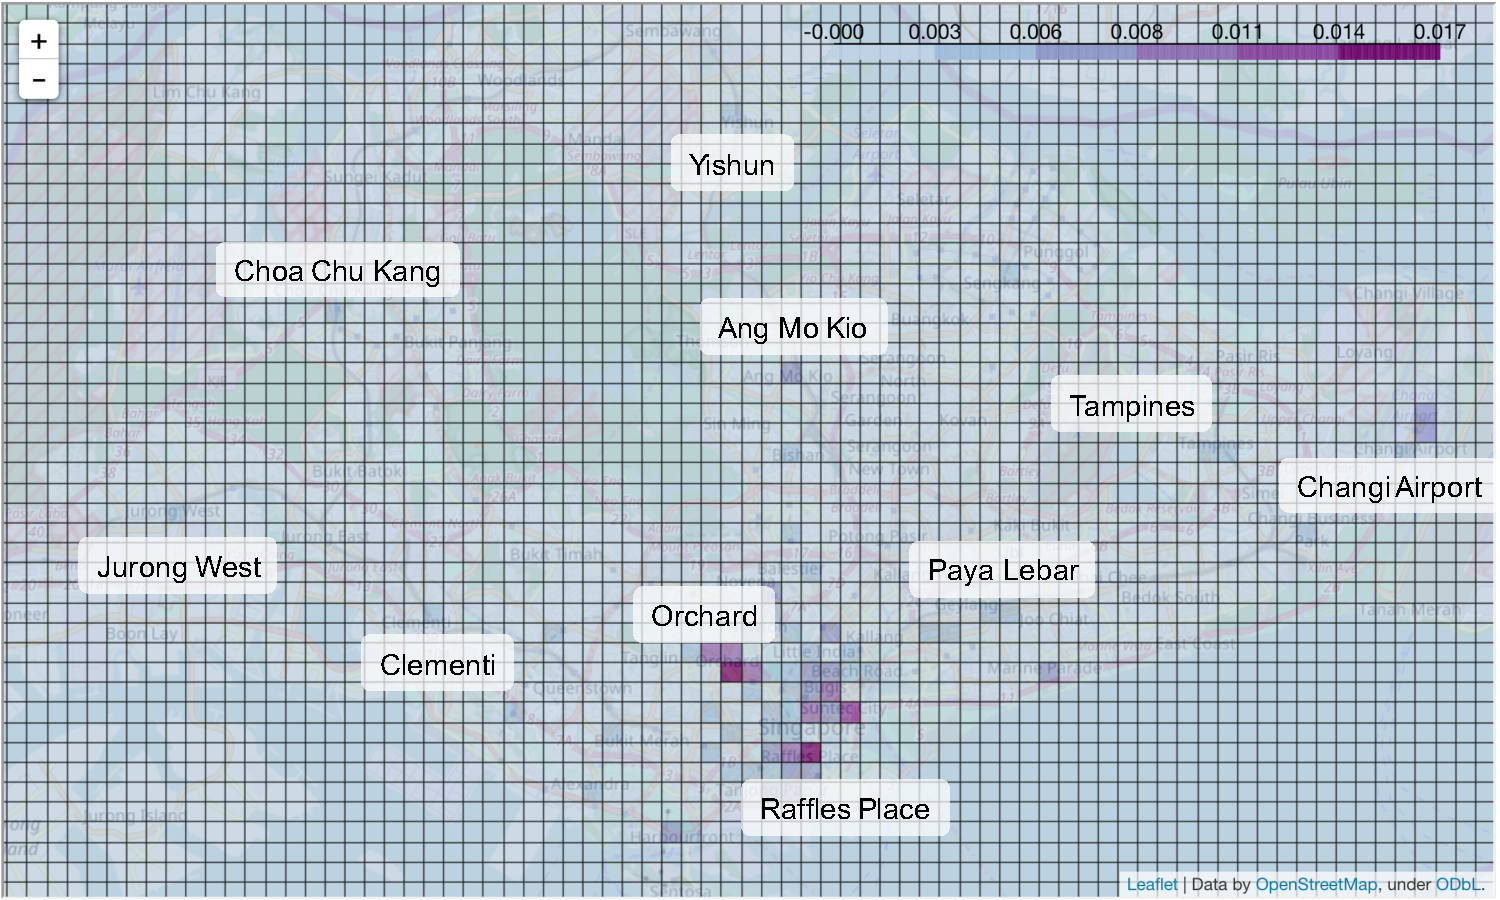
\includegraphics[width=0.95\linewidth]{figs/locationHeatMap}
  \caption{Pick-up location heat map}
  \label{fig:locationHeatMap}
\end{subfigure}

%\vspace{-0.3 cm}
\caption{Map of Singapore}
\label{fig:mapSingapore}
%\vspace{-0.5 cm}
\end{figure}


We split Singapore in a grid form, like Figure~\ref{fig:gridSingapore}, to manage trajectory history efficiently and define each cell as zones. The size of a cell is 0.5km by 0.5km. We consider that this size is enough to capture queueing time. Queueing time is defined roaming time for finding a passenger or waiting at a taxi stand. More details about quantifying queueing time are mentioned in Section 3. Figure~\ref{fig:locationHeatMap} shows general locations where taxi drivers pick up passengers often. Most of the trips occurred at city areas such as Orchard and Raffles Place. Removing homophily effect is a big issue in detecting active community. For example, many last mile trips, from a transportation hub to a final destination, occurs in a few locations such as Yishun and Tampines. Some drivers usually return the same location where they pick up passengers after they finish services. They show same trajectory patterns, but it is hard to define them as the same community because they just follow their preference without interaction with other drivers. Therefore, we need a systematic approach to detect real and active communities.



\section{Community detection framework} \label{sec:comDectectionFramework}


\begin{figure} [h]
  \centering
  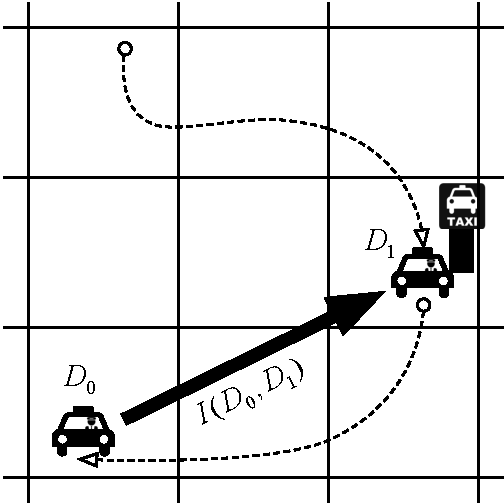
\includegraphics[width=0.8\linewidth]{figs/driverInfluence}
  \caption{Influence between drivers}
  \label{fig:driverInfluence}
\end{figure}



\subsection{Length of Papers}

Each accepted full paper is allocated six pages in the conference 
proceedings, excluded references. References can take up to one page.
Up to two additional pages may be purchased at a price 
to be announced per page for any accepted paper. However, all 
{\em submissions} must 
be a maximum of six pages, plus at most one for references, in length.


\subsection{Word Processing Software}

As detailed below, IJCAI has prepared and made available a set of
\LaTeX{} macros and a Microsoft Word template for use in formatting
your paper. If you are using some other word processing software (such
as WordPerfect, etc.), please follow the format instructions given
below and ensure that your final paper looks as much like this sample
as possible.

\section{Style and Format}

\LaTeX{} and Word style files that implement these instructions
can be retrieved electronically. (See Appendix~\ref{stylefiles} for
instructions on how to obtain these files.)

\subsection{Layout}

Print manuscripts two columns to a page, in the manner in which these
instructions are printed. The exact dimensions for pages are:
\begin{itemize}
\item left and right margins: .75$''$
\item column width: 3.375$''$
\item gap between columns: .25$''$
\item top margin---first page: 1.375$''$
\item top margin---other pages: .75$''$
\item bottom margin: 1.25$''$
\item column height---first page: 6.625$''$
\item column height---other pages: 9$''$
\end{itemize}

All measurements assume an 8-1/2$''$ $\times$ 11$''$ page size. For
A4-size paper, use the given top and left margins, column width,
height, and gap, and modify the bottom and right margins as necessary.

\subsection{Format of Electronic Manuscript}

For the production of the electronic manuscript, you must use Adobe's
{\em Portable Document Format} (PDF). A PDF file can be generated, for
instance, on Unix systems using {\tt ps2pdf} or on Windows systems
using Adobe's Distiller. There is also a website with free software
and conversion services: {\tt http://www.ps2pdf.com/}. For reasons of
uniformity, use of Adobe's {\em Times Roman} font is strongly suggested. In
\LaTeX2e{}, this is accomplished by putting
\begin{quote} 
\mbox{\tt $\backslash$usepackage\{times\}}
\end{quote}
in the preamble.\footnote{You may want also to use the package {\tt
latexsym}, which defines all symbols known from the old \LaTeX{}
version.}
  
Additionally, it is of utmost importance to specify the American {\bf
letter} format (corresponding to 8-1/2$''$ $\times$ 11$''$) when
formatting the paper. When working with {\tt dvips}, for instance, one
should specify {\tt -t letter}.

\subsection{Title and Author Information}

Center the title on the entire width of the page in a 14-point bold
font. Below it, center the author name(s) in a 12-point bold font, and
then center the address(es) in a 12-point regular font. Credit to a
sponsoring agency can appear on the first page as a footnote.

\subsubsection{Blind Review}

In order to make blind reviewing possible, authors must omit their
names and affiliations when submitting the paper for review. In place
of names and affiliations, provide a list of content areas. When
referring to one's own work, use the third person rather than the
first person. For example, say, ``Previously,
Gottlob~\shortcite{gottlob:nonmon} has shown that\ldots'', rather
than, ``In our previous work~\cite{gottlob:nonmon}, we have shown
that\ldots'' Try to avoid including any information in the body of the
paper or references that would identify the authors or their
institutions. Such information can be added to the final camera-ready
version for publication.

\subsection{Abstract}

Place the abstract at the beginning of the first column 3$''$ from the
top of the page, unless that does not leave enough room for the title
and author information. Use a slightly smaller width than in the body
of the paper. Head the abstract with ``Abstract'' centered above the
body of the abstract in a 12-point bold font. The body of the abstract
should be in the same font as the body of the paper.

The abstract should be a concise, one-paragraph summary describing the
general thesis and conclusion of your paper. A reader should be able
to learn the purpose of the paper and the reason for its importance
from the abstract. The abstract should be no more than 200 words long.

\subsection{Text}

The main body of the text immediately follows the abstract. Use
10-point type in a clear, readable font with 1-point leading (10 on
11).

Indent when starting a new paragraph, except after major headings.

\subsection{Headings and Sections}

When necessary, headings should be used to separate major sections of
your paper. (These instructions use many headings to demonstrate their
appearance; your paper should have fewer headings.)

\subsubsection{Section Headings}

Print section headings in 12-point bold type in the style shown in
these instructions. Leave a blank space of approximately 10 points
above and 4 points below section headings.  Number sections with
arabic numerals.

\subsubsection{Subsection Headings}

Print subsection headings in 11-point bold type. Leave a blank space
of approximately 8 points above and 3 points below subsection
headings. Number subsections with the section number and the
subsection number (in arabic numerals) separated by a
period.

\subsubsection{Subsubsection Headings}

Print subsubsection headings in 10-point bold type. Leave a blank
space of approximately 6 points above subsubsection headings. Do not
number subsubsections.

\subsubsection{Special Sections}

You may include an unnumbered acknowledgments section, including
acknowledgments of help from colleagues, financial support, and
permission to publish.

Any appendices directly follow the text and look like sections, except
that they are numbered with capital letters instead of arabic
numerals.

The references section is headed ``References,'' printed in the same
style as a section heading but without a number. A sample list of
references is given at the end of these instructions. Use a consistent
format for references, such as that provided by Bib\TeX{}. The reference
list should not include unpublished work.

\subsection{Citations}

Citations within the text should include the author's last name and
the year of publication, for example~\cite{gottlob:nonmon}.  Append
lowercase letters to the year in cases of ambiguity.  Treat multiple
authors as in the following examples:~\cite{abelson-et-al:scheme}
or~\cite{bgf:Lixto} (for more than two authors) and
\cite{brachman-schmolze:kl-one} (for two authors).  If the author
portion of a citation is obvious, omit it, e.g.,
Nebel~\shortcite{nebel:jair-2000}.  Collapse multiple citations as
follows:~\cite{gls:hypertrees,levesque:functional-foundations}.
\nocite{abelson-et-al:scheme}
\nocite{bgf:Lixto}
\nocite{brachman-schmolze:kl-one}
\nocite{gottlob:nonmon}
\nocite{gls:hypertrees}
\nocite{levesque:functional-foundations}
\nocite{levesque:belief}
\nocite{nebel:jair-2000}

\subsection{Footnotes}

Place footnotes at the bottom of the page in a 9-point font.  Refer to
them with superscript numbers.\footnote{This is how your footnotes
should appear.} Separate them from the text by a short
line.\footnote{Note the line separating these footnotes from the
text.} Avoid footnotes as much as possible; they interrupt the flow of
the text.

\section{Illustrations}

Place all illustrations (figures, drawings, tables, and photographs)
throughout the paper at the places where they are first discussed,
rather than at the end of the paper. If placed at the bottom or top of
a page, illustrations may run across both columns.

Illustrations must be rendered electronically or scanned and placed
directly in your document. All illustrations should be in black and
white, as color illustrations may cause problems. Line weights should
be 1/2-point or thicker. Avoid screens and superimposing type on
patterns as these effects may not reproduce well.

Number illustrations sequentially. Use references of the following
form: Figure 1, Table 2, etc. Place illustration numbers and captions
under illustrations. Leave a margin of 1/4-inch around the area
covered by the illustration and caption.  Use 9-point type for
captions, labels, and other text in illustrations.

\section*{Acknowledgments}

The preparation of these instructions and the \LaTeX{} and Bib\TeX{}
files that implement them was supported by Schlumberger Palo Alto
Research, AT\&T Bell Laboratories, and Morgan Kaufmann Publishers.
Preparation of the Microsoft Word file was supported by IJCAI.  An
early version of this document was created by Shirley Jowell and Peter
F. Patel-Schneider.  It was subsequently modified by Jennifer
Ballentine and Thomas Dean, Bernhard Nebel, and Daniel Pagenstecher.
These instructions are the same as the ones for IJCAI--05, prepared by
Kurt Steinkraus, Massachusetts Institute of Technology, Computer
Science and Artificial Intelligence Lab.

\appendix

\section{\LaTeX{} and Word Style Files}\label{stylefiles}

The \LaTeX{} and Word style files are available on the IJCAI--17
website, {\tt http://www.ijcai-17.org/}.
These style files implement the formatting instructions in this
document.

The \LaTeX{} files are {\tt ijcai17.sty} and {\tt ijcai17.tex}, and
the Bib\TeX{} files are {\tt named.bst} and {\tt ijcai17.bib}. The
\LaTeX{} style file is for version 2e of \LaTeX{}, and the Bib\TeX{}
style file is for version 0.99c of Bib\TeX{} ({\em not} version
0.98i). The {\tt ijcai17.sty} file is the same as the {\tt
ijcai07.sty} file used for IJCAI--07.

The Microsoft Word style file consists of a single file, {\tt
ijcai17.doc}. This template is the same as the one used for
IJCAI--07.

These Microsoft Word and \LaTeX{} files contain the source of the
present document and may serve as a formatting sample.  

Further information on using these styles for the preparation of
papers for IJCAI--17 can be obtained by contacting {\tt
pcchair@ijcai-17.org}.

%% The file named.bst is a bibliography style file for BibTeX 0.99c
\bibliographystyle{named}
\bibliography{ijcai17}

\end{document}

